\documentclass[11pt]{article}

% ── Packages ──────────────────────────────────────────────────────────────────
\usepackage{amsmath, amsthm, amssymb}
\usepackage{geometry}
\usepackage{graphicx}
\usepackage{tikz}
\usepackage{hyperref}
\usepackage{enumitem}
\usepackage{xcolor}
\usepackage{mdframed}
\usepackage{float}
\usepackage{algorithm}
\usepackage{algpseudocode}
\usepackage{algpseudocode}

\geometry{margin=1in}
\hypersetup{colorlinks=true, linkcolor=blue!60!black, urlcolor=blue!60!black}

% ── Theorem Environments ──────────────────────────────────────────────────────
\theoremstyle{plain}
\newtheorem{theorem}{Theorem}[section]
\newtheorem{lemma}[theorem]{Lemma}
\newtheorem{proposition}[theorem]{Proposition}
\newtheorem{example}[theorem]{Example}

\theoremstyle{definition}
\newtheorem{definition}[theorem]{Definition}
\newtheorem{remark}[theorem]{Remark}

% ── Macros ────────────────────────────────────────────────────────────────────
\newcommand{\Z}{\mathbb{Z}}
\newcommand{\R}{\mathbb{R}}
\newcommand{\norm}[1]{\left\lVert #1 \right\rVert}
\newcommand{\floor}[1]{\left\lfloor #1 \right\rfloor}


% ── Highlight box ─────────────────────────────────────────────────────────────
\newmdenv[
  backgroundcolor=blue!5,
  linecolor=blue!40,
  linewidth=1.2pt,
  roundcorner=4pt,
  skipabove=8pt,
  skipbelow=8pt
]{keybox}

\begin{document}

\noindent
\begin{tabular}{|p{0.72\textwidth} r|}
\hline
\textbf{Recreational Mathematics Club} & \textit{Discussion \#5} \\[4pt]
\multicolumn{2}{|c|}{\Large Matroids} \\[4pt]
Speaker: \textit{Mahek Shamsukha} & Indian Institute of Science \\
\hline
\end{tabular}


% ══════════════════════════════════════════════════════════════════════════════
\section{Examples and Motivation}
% ══════════════════════════════════════════════════════════════════════════════
 
We begin with three different notions of independence arising from
linear algebra, graph theory, and matching theory.
Remarkably, all three examples give rise to exactly the same collection
of independent sets.
 
\begin{enumerate}[label=\textbf{Example \arabic*.}, leftmargin=*, itemsep=1.2ex]
 
% ── Example 1 ───────────────────────────────────────────────────────────────────
\item \textbf{Linear Independence.}
 
Consider the vectors $a, b, c, d, e, f \in \mathbb{R}^{3}$ shown below.
 
\begin{center}
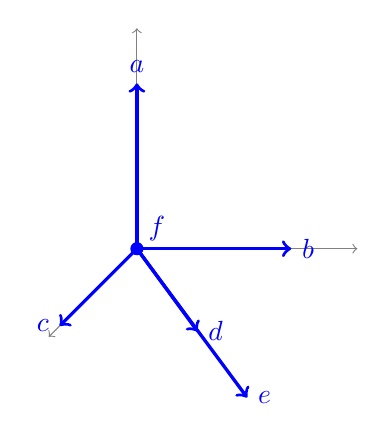
\begin{tikzpicture}[scale=1.4]
  \draw[->, gray] (0,0) -- (0,2);
  \draw[->, gray] (0,0) -- (2,0);
  \draw[->, gray] (0,0) -- (-0.8,-0.8);
 
  \draw[very thick, blue, ->] (0,0) -- (0,1.5)  node[above]       {$a$};
  \draw[very thick, blue, ->] (0,0) -- (1.4,0)   node[right]       {$b$};
  \draw[very thick, blue, ->] (0,0) -- (-0.7,-0.7) node[left]      {$c$};
  \draw[very thick, blue, ->] (0,0) -- (0.55,-0.75) node[right]    {$d$};
  \draw[very thick, blue, ->] (0,0) -- (1.0,-1.35)  node[right]    {$e$};
 
  \fill[blue] (0,0) circle (1.7pt);
  \node[blue] at (0.18,0.18) {$f$};
\end{tikzpicture}
\end{center}
 
A subset of $E = \{a,b,c,d,e,f\}$ is called \emph{independent} if the
corresponding vectors are linearly independent.
The maximal independent sets are
\[
  \{a,b,c\},\quad \{a,b,d\},\quad \{a,b,e\},\quad \{a,c,d\},\quad \{a,c,e\}.
\]
Hence the independent sets are exactly all subsets of these five sets.
For example, $\{a,b,d\}$ is independent, while $\{b,c,d,e\}$ is dependent.
Any set containing $f$ together with three nonzero vectors is dependent
since $f = 0$.
 
% ── Example 2 ───────────────────────────────────────────────────────────────────
\item \textbf{Acyclic Edge Sets.}
 
Consider the graph below with edge set $E = \{a,b,c,d,e,f\}$.
 
\begin{center}
\begin{tikzpicture}[scale=1.4]
  \node[circle, fill, inner sep=1.7pt] (v1) at (5,0)  {};
  \node[circle, fill, inner sep=1.7pt] (v2) at (2,0)  {};
  \node[circle, fill, inner sep=1.7pt] (v3) at (1,1)  {};
  \node[circle, fill, inner sep=1.7pt] (v4) at (1,-1) {};
 
  \draw (v1) -- node[below]       {$a$} (v2);
  \draw (v2) -- node[above right] {$b$} (v3);
  \draw (v2) -- node[below right] {$c$} (v4);
  \draw (v3) to[bend left=18]  node[right] {$d$} (v4);
  \draw (v3) to[bend right=18] node[left]  {$e$} (v4);
  \draw (v1) to[loop right=10] node        {$f$} (v1);
\end{tikzpicture}
\end{center}
 
A subset of edges is independent if it contains no cycle.
The maximal independent sets are again
\[
  \{a,b,c\},\quad \{a,b,d\},\quad \{a,b,e\},\quad \{a,c,d\},\quad \{a,c,e\}.
\]
These are precisely the spanning trees of the graph.
For example, $\{a,b,d\}$ is independent, while $\{b,c,d\}$ is dependent
since it forms a cycle.
Any set containing the loop $f$ is dependent.
 
% ── Example 3 ───────────────────────────────────────────────────────────────────
\item \textbf{Matchings / Systems of Distinct Representatives.}
 
Consider the bipartite graph below.
 
\begin{center}
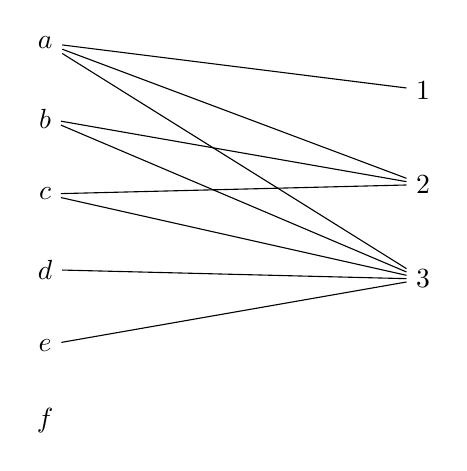
\begin{tikzpicture}[scale=1.2]
  \node (1) at (4,2)    {$1$};
  \node (2) at (4,1)    {$2$};
  \node (3) at (4,0)    {$3$};
 
  \node (a) at (0, 2.5) {$a$};
  \node (b) at (0, 1.7) {$b$};
  \node (c) at (0, 0.9) {$c$};
  \node (d) at (0, 0.1) {$d$};
  \node (e) at (0,-0.7) {$e$};
  \node (f) at (0,-1.5) {$f$};
 
  \draw (a)--(1); \draw (a)--(2); \draw (a)--(3);
  \draw (b)--(2); \draw (b)--(3);
  \draw (c)--(2); \draw (c)--(3);
  \draw (d)--(3);
  \draw (e)--(3);
\end{tikzpicture}
\end{center}
 
Define
\[
  A_1 = \{a\},\qquad A_2 = \{a,b,c\},\qquad A_3 = \{a,b,c,d,e\}.
\]
A subset of $E = \{a,b,c,d,e,f\}$ is called independent if it admits a
system of distinct representatives, or equivalently, if it can be saturated
by a matching.
The maximal independent sets are once again
\[
  \{a,b,c\},\quad \{a,b,d\},\quad \{a,b,e\},\quad \{a,c,d\},\quad \{a,c,e\}.
\]
For example, $\{a,c,d\}$ is independent since we can match
$a \to 1$, $c \to 2$, $d \to 3$.
However, $\{b,c,d\}$ is dependent because all three sets are contained in
$\{2,3\}$, so Hall's condition fails.
The element $f$ is dependent by itself since it has no neighbour.
 
\end{enumerate}
 
Thus, although the three examples come from very different areas of
mathematics, they define exactly the same family of independent subsets of
$E = \{a,b,c,d,e,f\}$.
This common abstract structure is called a \emph{matroid}.
 
% ══════════════════════════════════════════════════════════════════════════════
\section{Hereditary Set Systems}
% ══════════════════════════════════════════════════════════════════════════════
 
\begin{definition}
Let $E$ be a finite set and let $\mathcal{F} \subseteq 2^{E}$.
The pair $(E, \mathcal{F})$ is a \emph{hereditary set system} if
\[
  \forall\, A \in \mathcal{F},\; \forall\, A' \subseteq A
  \implies A' \in \mathcal{F}.
\]
\end{definition}
 
\begin{example}
The following are hereditary set systems.
\begin{enumerate}[leftmargin=*, itemsep=0.6ex]
 
\item Let $G = (V,E)$ be a graph and $\mathcal{F} = \{F \subseteq E : F
      \text{ contains no cycle}\}$.
 
\item Let $G = (V,E)$ be a graph and $\mathcal{F} = \{M \subseteq E : M
      \text{ is a matching}\}$.
 
\item Let $G = (V,E)$ be a graph and $\mathcal{F} = \{S \subseteq V : S
      \text{ induces a clique}\}$.
 
\item Let $G = (V,E)$ be a graph and $\mathcal{F} = \{S \subseteq V : S
      \text{ is an independent set}\}$.
 
\item Let $E = \{1,\dots,n\}$ and fix an integer $k$. Define
      $\mathcal{F} = \{S \subseteq E : |S| \le k\}$.
 
\item Let $E = \{1,\dots,n\}$ and define
      $\mathcal{F} = \bigl\{S \subseteq E : \sum_{i \in S} i \le 10\bigr\}$.
 
      However, this need not be a matroid.
      For example, $\{10\}, \{4,5\} \in \mathcal{F}$ with $|\{10\}| < |\{4,5\}|$,
      yet neither $\{10,4\}$ nor $\{10,5\}$ belongs to $\mathcal{F}$,
      so the exchange property fails.
 
\end{enumerate}
\end{example}
 
% ══════════════════════════════════════════════════════════════════════════════
\section{Matroids}
% ══════════════════════════════════════════════════════════════════════════════
 
\begin{definition}
A \emph{matroid} is a pair $M = (E, \mathcal{I})$, where $E$ is a finite set
and $\mathcal{I} \subseteq 2^{E}$ is a collection of \emph{independent sets},
satisfying:
\begin{enumerate}[label=(\roman*), itemsep=0.4ex]
  \item $\emptyset \in \mathcal{I}$.
  \item If $I \in \mathcal{I}$ and $I' \subseteq I$, then $I' \in \mathcal{I}$.
  \item \textbf{(Exchange axiom)} If $I_1, I_2 \in \mathcal{I}$ and $|I_1| < |I_2|$,
        then there exists $e \in I_2 \setminus I_1$ such that
        $I_1 \cup \{e\} \in \mathcal{I}$.
\end{enumerate}
\end{definition}
 
\begin{example}
Let
\[
  A = \begin{pmatrix} 1 & 0 & 1 & 1 \\ 0 & 1 & 1 & 2 \end{pmatrix},
\]
and let $E = \{1,2,3,4\}$, where element $i$ corresponds to the $i$-th column
of $A$. Define $\mathcal{I}$ to consist of those $S \subseteq E$ for which the
columns indexed by $S$ are linearly independent.
 
Then $(E, \mathcal{I})$ is a matroid. For example, $\{1,2\}$, $\{1,4\}$, and
$\{2,3\}$ are independent, while $\{1,2,3\}$ is dependent. For instance:
\[
\begin{pmatrix}1\\1\end{pmatrix} = \begin{pmatrix}1\\0\end{pmatrix} + \begin{pmatrix}0\\1\end{pmatrix}
\]
\end{example}
 
\begin{proposition}
Let $A$ be a matrix with column set $E$, and let
$\mathcal{I} = \{S \subseteq E : S \text{ is linearly independent}\}$.
Then $(E, \mathcal{I})$ is a matroid.
\end{proposition}
 
\begin{proof}
We verify the matroid axioms.
\begin{enumerate}[label=(\roman*), itemsep=0.4ex]
  \item $\emptyset \in \mathcal{I}$.
  \item Every subset of a linearly independent set is linearly independent.
  \item Let $I_1, I_2 \in \mathcal{I}$ with $|I_1| < |I_2|$.
        If every $e \in I_2 \setminus I_1$ satisfies
        $I_1 \cup \{e\} \notin \mathcal{I}$, then every column in
        $I_2 \setminus I_1$ lies in $\operatorname{span}(I_1)$,
        so $\operatorname{span}(I_2) \subseteq \operatorname{span}(I_1)$,
        giving $|I_2| = \dim(\operatorname{span}(I_2))
        \le \dim(\operatorname{span}(I_1)) = |I_1|$, a contradiction. \qedhere
\end{enumerate}
\end{proof}
 
% ══════════════════════════════════════════════════════════════════════════════
\section{Bases}
% ══════════════════════════════════════════════════════════════════════════════
 
\begin{definition}
A set $B \in \mathcal{I}$ is a \emph{basis} of a matroid $M = (E, \mathcal{I})$
if it is maximal with respect to inclusion, i.e.\
$B \cup \{e\} \notin \mathcal{I}$ for all $e \in E \setminus B$.
\end{definition}
 
\begin{proposition}
All bases of a matroid have the same cardinality.
\end{proposition}
 
\begin{proof}
Let $B_1, B_2$ be bases with $|B_1| < |B_2|$.
By the exchange axiom there exists $e \in B_2 \setminus B_1$ such that
$B_1 \cup \{e\} \in \mathcal{I}$, contradicting the maximality of $B_1$.
\end{proof}
 
\begin{theorem}
Let $\mathcal{B} \subseteq 2^{E}$ be a nonempty collection of subsets of $E$.
Then $\mathcal{B}$ is the collection of bases of a matroid if and only if:
\begin{enumerate}[label=(\roman*), itemsep=0.4ex]
  \item $|B_1| = |B_2|$ for all $B_1, B_2 \in \mathcal{B}$.
  \item For all $B_1, B_2 \in \mathcal{B}$ and $e \in B_1 \setminus B_2$,
        there exists $f \in B_2 \setminus B_1$ such that
        $(B_1 \setminus \{e\}) \cup \{f\} \in \mathcal{B}$.
\end{enumerate}
\end{theorem}
 
\begin{proof}
$(\Rightarrow)$ If $\mathcal{B}$ is the collection of bases of a matroid,
all bases have the same size by the preceding proposition, and the exchange
property follows from the matroid axioms.
 
$(\Leftarrow)$ Define
\[
  \mathcal{I} = \{I \subseteq E : I \subseteq B \text{ for some } B \in \mathcal{B}\}.
\]
Clearly $\mathcal{I}$ is hereditary.
We verify the exchange axiom.
Let $I_1, I_2 \in \mathcal{I}$ with $|I_1| < |I_2|$, and suppose for
contradiction that $I_1 \cup \{e\} \notin \mathcal{I}$ for every
$e \in I_2 \setminus I_1$.
 
Choose $B_1 \supseteq I_1$ and $B_2 \supseteq I_2$ in $\mathcal{B}$.
Applying the basis exchange property repeatedly, we replace elements of
$B_2 \setminus (B_1 \cup I_2)$ by elements of $B_1 \setminus B_2$,
obtaining a new basis $B_2$ with $B_2 \setminus B_1 = I_2 \setminus B_1$.
Our assumption implies $I_2 \setminus B_1 = I_2 \setminus I_1$
(if there existed $e \in (I_2 \cap B_1) \setminus I_1$ then
$I_1 \cup \{e\} \subseteq B_1$ would give $I_1 \cup \{e\} \in \mathcal{I}$,
a contradiction).
Hence
\[
  |B_2 \setminus B_1| = |I_2 \setminus I_1| > |I_1 \setminus I_2|
  \ge |B_1 \setminus B_2|,
\]
contradicting $|B_1| = |B_2|$.
\end{proof}
 
\begin{example}
Let $G = (V,E)$ be a graph and $\mathcal{B}$ be the collection of spanning
forests of $G$.
\begin{enumerate}[label=(\roman*), itemsep=0.4ex]
  \item All spanning forests have the same size $|V| - c(G)$, where $c(G)$
        denotes the number of connected components.
  \item Let $F_1, F_2 \in \mathcal{B}$ and $e \in F_1 \setminus F_2$.
        Removing $e$ from $F_1$ splits one tree into two components $A$ and $B$.
        Since $F_2$ is a spanning forest, there must exist
        $f \in F_2 \setminus F_1$ with one endpoint in $A$ and the other in $B$;
        then $(F_1 \setminus \{e\}) \cup \{f\}$ is again a spanning forest.
\end{enumerate}
Hence the spanning forests of $G$ form the bases of a matroid whose
independent sets are exactly the acyclic edge subsets of $G$.
\end{example}
 
\begin{example}[Uniform Matroids]
Let $E$ be a finite set and $k$ a nonnegative integer. The pair
\[
  (E,\; \mathcal{I}) \quad\text{with}\quad
  \mathcal{I} = \{S \subseteq E : |S| \le k\}
\]
is a matroid, called the \emph{uniform matroid} $U_{k,E}$.
\end{example}
 
\begin{example}[Transversal Matroids]
Let $A_1, \dots, A_m \subseteq E$.
A subset $S \subseteq E$ is independent if it admits a system of distinct
representatives from $A_1, \dots, A_m$.
The resulting matroid is called a \emph{transversal matroid}.
\end{example}
 
% ══════════════════════════════════════════════════════════════════════════════
\section{Greedy Algorithm}
% ══════════════════════════════════════════════════════════════════════════════
 
Let $(E, \mathcal{I})$ be a hereditary set system and $w : E \to \mathbb{R}$
a weight function.
We assume access to an \emph{independence oracle}: given $S \subseteq E$,
we can determine whether $S \in \mathcal{I}$.
 
\begin{algorithm}[H]
\caption{\texttt{Greedy}$(E, w, \mathcal{I})$}
\begin{algorithmic}[1]
    \State \textbf{Input:} Finite set $E$, weight function $w : E \to \mathbb{R}$, independence oracle for $\mathcal{I}$
    \State \textbf{Output:} A maximum-weight maximal independent set $S \in \mathcal{I}$
    \State Sort $E = \{e_1, \dots, e_n\}$ so that $w(e_1) \geq w(e_2) \geq \cdots \geq w(e_n)$
    \State $S \gets \emptyset$
    \For{$i \gets 1$ \textbf{to} $n$}
        \If{$S \cup \{e_i\} \in \mathcal{I}$}
            \State $S \gets S \cup \{e_i\}$
        \EndIf
    \EndFor
    \State \Return{$S$}
\end{algorithmic}
\end{algorithm}
 
\begin{theorem}
Let $(E, \mathcal{I})$ be a hereditary set system with $\mathcal{I} \neq \emptyset$.
Then
\[
  (E, \mathcal{I}) \text{ is a matroid}
  \iff
  \forall\, w : E \to \mathbb{R},\quad
  w\!\left(\textsc{Greedy}(E,w,\mathcal{I})\right)
  = \max\!\bigl\{w(I) : I \in \mathcal{I},\; I \text{ maximal}\bigr\}.
\]
\end{theorem}
 
\begin{proof}
$(\Rightarrow)$
Assume $(E, \mathcal{I})$ is a matroid.
Call $Y \in \mathcal{I}$ \emph{good} if it is contained in some
maximum-weight basis.
We show that if $Y$ is good and the greedy algorithm next selects
$x \in E \setminus Y$, then $Y \cup \{x\}$ is also good.
 
Let $B$ be a maximum-weight basis with $Y \subseteq B$.
If $x \in B$, then $Y \cup \{x\} \subseteq B$ and we are done.
Suppose $x \notin B$.
 
\medskip\noindent
\textbf{Case 1:} $|B| = |Y \cup \{x\}|$, so $Y \cup \{x\}$ is itself a basis.
Since greedy chose $x$ as the heaviest element extendable from $Y$,
$w(x) \ge w(e)$ for all $e \in B \setminus Y$, hence
$w(Y \cup \{x\}) \ge w(B)$.
As $B$ is maximum-weight, $Y \cup \{x\}$ is also a maximum-weight basis.
 
\medskip\noindent
\textbf{Case 2:} $|B| > |Y \cup \{x\}|$.
Extend $Y \cup \{x\}$ to a basis $B'$ using elements of $B$;
then $Y \cup \{x\} \subseteq B' \subseteq B \cup \{x\}$.
Since $|B'| = |B|$, we have $B' = (B \cup \{x\}) \setminus \{x'\}$
for some $x' \in B \setminus Y$.
Because greedy selected $x$ before $x'$, $w(x) \ge w(x')$, so
$w(B') = w(B) - w(x') + w(x) \ge w(B)$.
Hence $B'$ is a maximum-weight basis containing $Y \cup \{x\}$.
 
\medskip
$(\Leftarrow)$
Suppose the greedy algorithm is optimal for every weight function
$w : E \to \mathbb{R}$.
Assume for contradiction that there exist $I_1, I_2 \in \mathcal{I}$ with
$|I_1| < |I_2|$ and $I_1 \cup \{e\} \notin \mathcal{I}$ for all
$e \in I_2 \setminus I_1$.
 
Choose $\varepsilon \in \mathbb{R}$ satisfying
\[
  \frac{|I_1| - |I_2 \cap I_1|}{|I_2| - |I_2 \cap I_1|} < \varepsilon < 1,
\]
and define $w : E \to \mathbb{R}$ by
\[
  w(e) = \begin{cases}
    1          & e \in I_1, \\
    \varepsilon & e \in I_2 \setminus I_1, \\
    0          & \text{otherwise.}
  \end{cases}
\]
The greedy algorithm selects all of $I_1$ first and, by assumption, cannot
add any element of $I_2 \setminus I_1$, so $w(S_G) = |I_1|$.
Extending $I_2$ to a maximal independent set $I_2'$ gives
\[
  w(I_2') \ge |I_1 \cap I_2| + \varepsilon|I_2 \setminus I_1|
           > |I_1| = w(S_G),
\]
contradicting optimality.
Hence the exchange axiom holds and $(E, \mathcal{I})$ is a matroid.
\end{proof}
 
% ══════════════════════════════════════════════════════════════════════════════
\section{Representable and Graphic Matroids}
% ══════════════════════════════════════════════════════════════════════════════
 
\begin{definition}
A matroid $M = (E, \mathcal{I})$ is \emph{representable over a field
$\mathbb{F}$} if there exists a matrix $A$ over $\mathbb{F}$ with columns
indexed by $E$ such that $S \subseteq E$ is independent in $M$ if and only if
the corresponding columns of $A$ are linearly independent.
\end{definition}
 
\begin{definition}
Let $G = (V,E)$ be a graph.
The \emph{graphic matroid} of $G$ is the matroid whose independent sets are
the acyclic subsets of $E$.
\end{definition}
 
\begin{theorem}
Every graphic matroid is representable over $\mathbb{R}$.
\end{theorem}
 
\begin{proof}
Let $V = \{v_1, \dots, v_n\}$.
Orient each edge of $G$ arbitrarily, and construct
$A \in \mathbb{R}^{V \times E}$ by setting, for each edge $e = (u,v)$
directed from $u$ to $v$, the column $c_e$ to have $+1$ in row $u$,
$-1$ in row $v$, and $0$ elsewhere.
 
We claim that a set of edges is linearly independent if and only if it
is acyclic.
If $e_1, \dots, e_k$ form a cycle, orienting it cyclically yields
$c_{e_1} + \cdots + c_{e_k} = 0$, so the columns are dependent.
Conversely, if the edge set contains no cycle then each component is a
tree; repeatedly removing a leaf shows inductively that all columns are
linearly independent.
\end{proof}
 
\begin{definition}
A matroid is \emph{regular} if it is representable over every field.
\end{definition}
 
\begin{remark}
The proof above works over any field (replace $-1$ by the additive inverse
of $1$), so every graphic matroid is regular.
\end{remark}
 
\begin{example}[Uniform Matroids]
The uniform matroid $U_{k,n}$ is representable over sufficiently large fields.
For instance, $U_{2,4}$ is represented over $\mathbb{R}$ by
\[
  \begin{pmatrix} 1 & 0 & 1 & 1 \\ 0 & 1 & 1 & 2 \end{pmatrix},
\]
since every pair of columns is linearly independent.
More generally, over an infinite field, choose $n$ distinct points on the
moment curve $(1, t, t^2, \dots, t^{k-1})$; any $k$ corresponding columns
are linearly independent.
\end{example}
 
\begin{example}
Uniform matroids need not be regular.
$U_{2,4}$ would require four nonzero vectors in $\mathbb{F}_2^2$
such that every pair is linearly independent, but $\mathbb{F}_2^2$ contains
only three nonzero vectors: $(1,0)$, $(0,1)$, $(1,1)$.
Hence $U_{2,4}$ is not representable over $\mathbb{F}_2$.
\end{example}
 
% ══════════════════════════════════════════════════════════════════════════════
\section{Restriction and Union of Matroids}
% ══════════════════════════════════════════════════════════════════════════════
 
\subsection{Restriction}
 
Let $M = (E, \mathcal{I})$ be a matroid and $A \subseteq E$.
The \emph{restriction} of $M$ to $A$ is
\[
  M|A = (A,\; \mathcal{I}|A), \qquad
  \mathcal{I}|A = \{I \in \mathcal{I} : I \subseteq A\}.
\]
 
\begin{theorem}
$M|A$ is a matroid on ground set $A$.
\end{theorem}
 
\begin{proof}
\emph{Non-emptiness:} $\emptyset \in \mathcal{I}$ and $\emptyset \subseteq A$,
so $\emptyset \in \mathcal{I}|A$.
\emph{Hereditary property:} If $I \in \mathcal{I}|A$ and $J \subseteq I$,
then $J \in \mathcal{I}$ and $J \subseteq A$, so $J \in \mathcal{I}|A$.
\emph{Exchange property:} Let $I, J \in \mathcal{I}|A$ with $|I| < |J|$.
Since $\mathcal{I}$ is a matroid, there exists $e \in J \setminus I$ with
$I \cup \{e\} \in \mathcal{I}$.
As $I, J \subseteq A$ we have $e \in A$, so $I \cup \{e\} \in \mathcal{I}|A$.
\end{proof}
 
\subsection{Union}
 
Let $M_1 = (E, \mathcal{I}_1)$ and $M_2 = (E, \mathcal{I}_2)$ be matroids on
the same ground set $E$, and define
\[
  \mathcal{I} = \{I_1 \cup I_2 : I_1 \in \mathcal{I}_1,\; I_2 \in \mathcal{I}_2\}.
\]
 
\begin{theorem}[Edmonds' Matroid Union Theorem]
$(E, \mathcal{I})$ is a matroid.
More generally, the union of finitely many matroids on $E$ is a matroid.
\end{theorem}
 
\begin{remark}
The set-theoretic union $\mathcal{I}_1 \cup \mathcal{I}_2$ of two independence
families is \emph{not} necessarily a matroid; the correct construction is the
family of unions of independent sets as defined above.
\end{remark}
 
\begin{example}[Partition Matroid]
Let $E = E_1 \sqcup E_2 \sqcup \cdots \sqcup E_k$ and fix integers
$0 \le r_i \le |E_i|$.
Call $I \subseteq E$ independent if $|I \cap E_i| \le r_i$ for all $i$.
The resulting matroid is called a \emph{partition matroid}.
 
For example, let $E = \{a,b,c,d,e,f\}$, $E_1 = \{a,b\}$,
$E_2 = \{c,d,e,f\}$, $r_1 = 1$, $r_2 = 2$.
Then $\{a,c,d\}$ is independent, while $\{a,b,c\}$ is not.
 
A partition matroid arises by taking the uniform matroid $U_{r_i,E}$ for
each block, restricting it to $E_i$, and forming the union of these
restricted matroids — so it is indeed a matroid by the preceding results.
\end{example}
 
 
\begin{thebibliography}{9}
 
\bibitem{oxley}
J.~G. Oxley,
\textit{Matroid Theory}, 2nd ed.
Oxford University Press, 2011.
Available at \url{https://www.math.ens.psl.eu/~benoist/refs/Oxley.pdf}.
 
\bibitem{goemans-lec9}
M.~X. Goemans (lecturer), B.~E. Tenner (scribe),
\textit{18.997 Topics in Combinatorial Optimization, Lecture 9: Matroids}.
MIT OpenCourseWare, Spring 2004.
\url{https://ocw.mit.edu/courses/18-997-topics-in-combinatorial-optimization-spring-2004/e93e0010583c4d9de9ee306b4cfee4e4_co_lec9.pdf}.
 
\bibitem{goemans-lec10}
M.~X. Goemans (lecturer), N.~Immorlica (scribe),
\textit{18.997 Topics in Combinatorial Optimization, Lecture 10: Matroid Representation and Optimization}.
MIT OpenCourseWare, Spring 2004.
\url{https://ocw.mit.edu/courses/18-997-topics-in-combinatorial-optimization-spring-2004/6faef8afbcaec34e49dd0dab12611e0f_co_lec10.pdf}.
 
\bibitem{iitd}
A.~Rai,
\textit{Lecture 13: Matroids}.
IIT Delhi, Course Lecture Notes.
\url{https://web.iitd.ac.in/~raiashutosh/Courses/lectures/lec13.pdf}.
 
\bibitem{ardila-lec1}
F.~Ardila,
\textit{Lecture 1 -- Matroids} [video lecture].
San Francisco State University / Universidad de Los Andes, 2007.
\url{https://www.youtube.com/watch?v=pe5MaEugAwg}.
 
\bibitem{ardila-lec4}
F.~Ardila,
\textit{Lecture 4 -- Matroids: Greedy Algorithm} [video lecture].
San Francisco State University / Universidad de Los Andes, 2007.
\url{https://www.youtube.com/watch?v=H4DoReLpGQk}.
 
\bibitem{imsc}
\textit{Lecture 15 -- Paraterized Complexity: Introduction to Matroids} [video lecture].
July 2020.
\url{https://www.youtube.com/watch?v=H4DoReLpGQk}.
 
\bibitem{fajardo}
L.~Fajardo Gomez,
\textit{Introduction to Matroids} [video lecture].
July 2020.
\url{https://www.youtube.com/watch?v=SljIEkfzloA}.
 
\end{thebibliography}
 
\end{document}



